\section{Tank Mixing Problem}
\label{sec:tank_mixing_problem}	

\subsection*{Recommended Tutorials:}
\begin{itemize}[noitemsep]
    \item \nameref{chp:equation_solvers}, pg. \pageref{chp:equation_solvers}
    \item \nameref{chp:limits}, pg. \pageref{chp:limits}
        \index{limit!}
	\item \nameref{chp:differential_equations}, pg. \pageref{chp:differential_equations}
	    \index{differential equations!}
\end{itemize}

\subsection*{Introduction:}
\marginnote[-1cm]{Concentration is defined as \[\text{concentration}=\frac{\text{mass}}{\text{volume}}.\] If we wish to determine mass, then we can rearrange the equation to obtain \[\text{mass}=\text{concentration}\times\text{volume}.\]}
Suppose you are having a wedding and you start with a $5$ L tank of coffee that has a concentration of \SI{60}{\gram/\liter}. The wedding guests are drinking the coffee at a rate of \SI{0.2}{\liter/\minute}. You are refilling the tank at a rate of \SI{0.15}{\liter/\minute} with coffee of a concentration of \SI{50}{\gram/\liter}.

\tikzset{
   ragged border/.style={ decoration={random steps, segment length=1mm, amplitude=0.5mm},
           decorate,
   }
}
\begin{figure}[h]
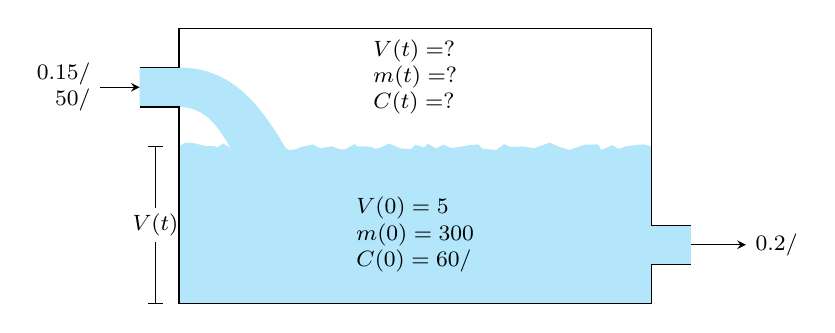
\begin{tikzpicture}
    \fill[cyan!30]
    decorate[ragged border]{
        (0,2) -- (6,2)
    }
    -- (6,1) -- (6.5,1) -- (6.5,0.5) -- (6,0.5) --(6,0) -- (0,0) -- cycle;
    \fill[cyan!30] (-0.5,2.5) -- (0,2.5) to[in=120,out=0](0.7,1.9)-- (1.4,1.9)
                  to[out=120,in=0] (0,3) -- (-0.5,3) -- cycle;
    \draw (-0.5,2.5) -- (0,2.5) -- (0,0) -- (6,0) -- (6,0.5) -- (6.5,0.5);
    \draw (-0.5,3) -- (0,3) -- (0,3.5) -- (6,3.5) -- (6,1) -- (6.5,1);
    \draw[|-|] (-0.3,0) --
        node[fill=white,font=\footnotesize,inner ysep=2pt,inner
                xsep=0]{$V(t)$}(-0.3,2);
    \draw[stealth-] (-0.5,2.75) -- (-1,2.75)
            node[anchor=east,font=\footnotesize,align=right]{\SI{0.15}{\liter/\minute}\\\SI{50}{\gram/\liter}};
    \draw[-stealth] (6.5,0.75) -- (7.2,0.75)
            node[anchor=west,font=\footnotesize]{\SI{0.2}{\liter/\minute}};
    \node[anchor=north,font=\footnotesize] at (3,3.5) {
        $\begin{array}{l}
             V(t)=? \\
             m(t)=? \\
             C(t)=?
        \end{array}$
    };
    \node[anchor=north,font=\footnotesize] at (3,1.5) {
        $\begin{array}{l}
             V(0)=\SI{5}{\liter}  \\
             m(0)=\SI{300}{\gram} \\
             C(0)=\SI{60}{\gram/\liter}
        \end{array}$
    };
\end{tikzpicture}
\caption{An illustration of the tank of coffee. The initial conditions for the volume and mass of coffee are shown.}
\label{fig:coffe_tank}
\end{figure}
\vspace{-1.4cm}

\subsection*{Exercises:}

\begin{enumerate}
\item 
\begin{enumerate}
    \item Setup a differential equation for the volume of coffee in the tank using $V'(t) = (\text{rate in}) - (\text{rate out}).$
    \item Solve this differential equation using the initial condition to obtain a formula for the volume $V(t)$ after $t$ minutes.
    \item Use the \texttt{solve()}\index{solving equations!solve} command to compute how long it will be until you run out of coffee.
\end{enumerate}
\item 
\begin{enumerate}
    \item Set up a differential equation for the mass of coffee in the tank using 
    \[m'(t) = \lrp{\begin{array}{l}
         \text{concentration}  \\
         \text{entering tank} 
    \end{array}}
    \lrp{\begin{array}{l}
         \text{volume}  \\
         \text{rate in} 
    \end{array}}
    -
    \lrp{\begin{array}{l}
         \text{concentration}  \\
         \text{in tank at time }t 
    \end{array}}
    \lrp{\begin{array}{l}
         \text{volume}  \\
         \text{rate out} 
    \end{array}}.\]
    \item Solve the differential equation for mass using your initial condition for the mass of the coffee $m(t)$ after $t$ minutes.
\end{enumerate}
\item Determine the function for the concentration of the coffee in the tank $C(t)$ after $t$ minutes using $C(t) = m(t)/V(t)$.
\item Plot $V(t)$, $m(t)$, and $C(t)$ on separate graphs to see what happens to the mass, volume, and concentration over time.
\item Use the \texttt{limit()}\index{limit} command to determine the concentration of coffee as you approach the last drop of coffee.
\end{enumerate}